%%  Figures of methodology


\begin{figure}
	\centering
	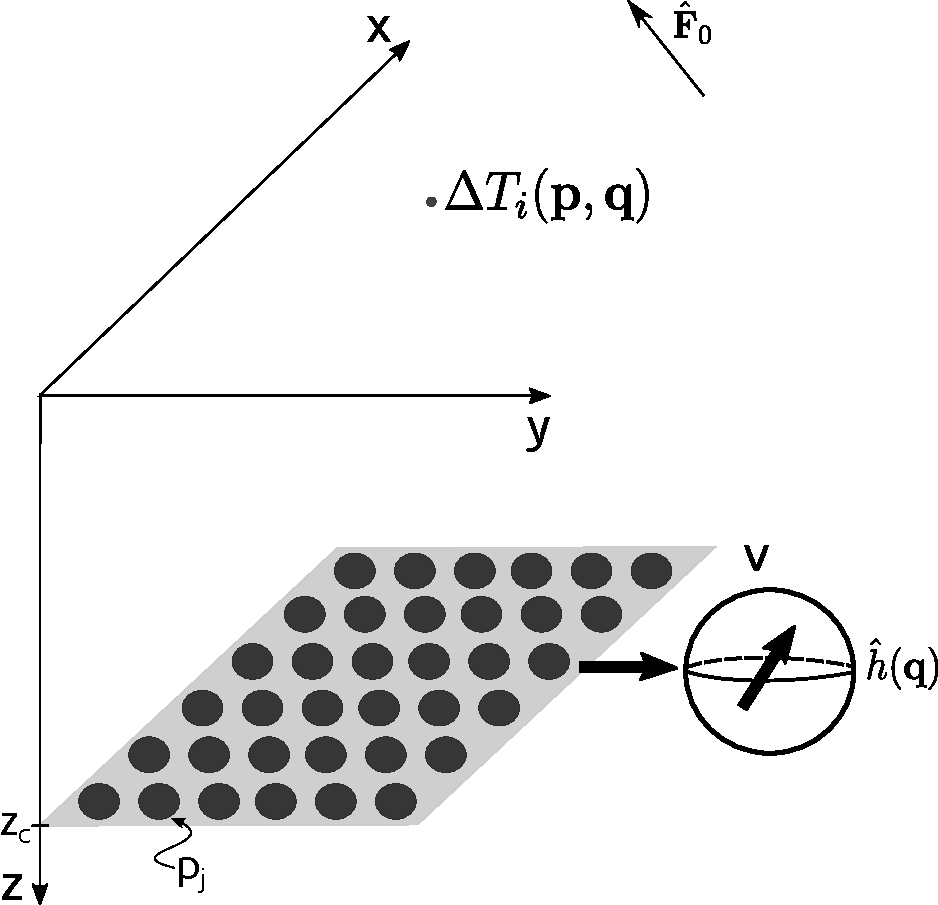
\includegraphics[width=0.7\textwidth]{Fig/eqlayer_figure.pdf}
	\caption{Schematic representation of an equivalent layer. The layer is positioned over the horizontal plane at a depth of $z=z_c$. $\Delta T_i =  f_i (\mathbf{s})$ is the predicted total-field anomaly at the point $(x_i,y_i,z_i)$ produced by the set of $M$ equivalent sources (black dots). Each source is located at the point $(x_j,y_j,z_c)$, $j = 1,\hdots, M$, and represented by a dipole with unity volume $\upsilon$ with magnetization direction $\hat{\mathbf{m}}(\mathbf{q})$ and magnetic moment $p_j$.    }
	\label{fig:eqlayer_figure}
\end{figure}


\begin{figure}
	\centering
	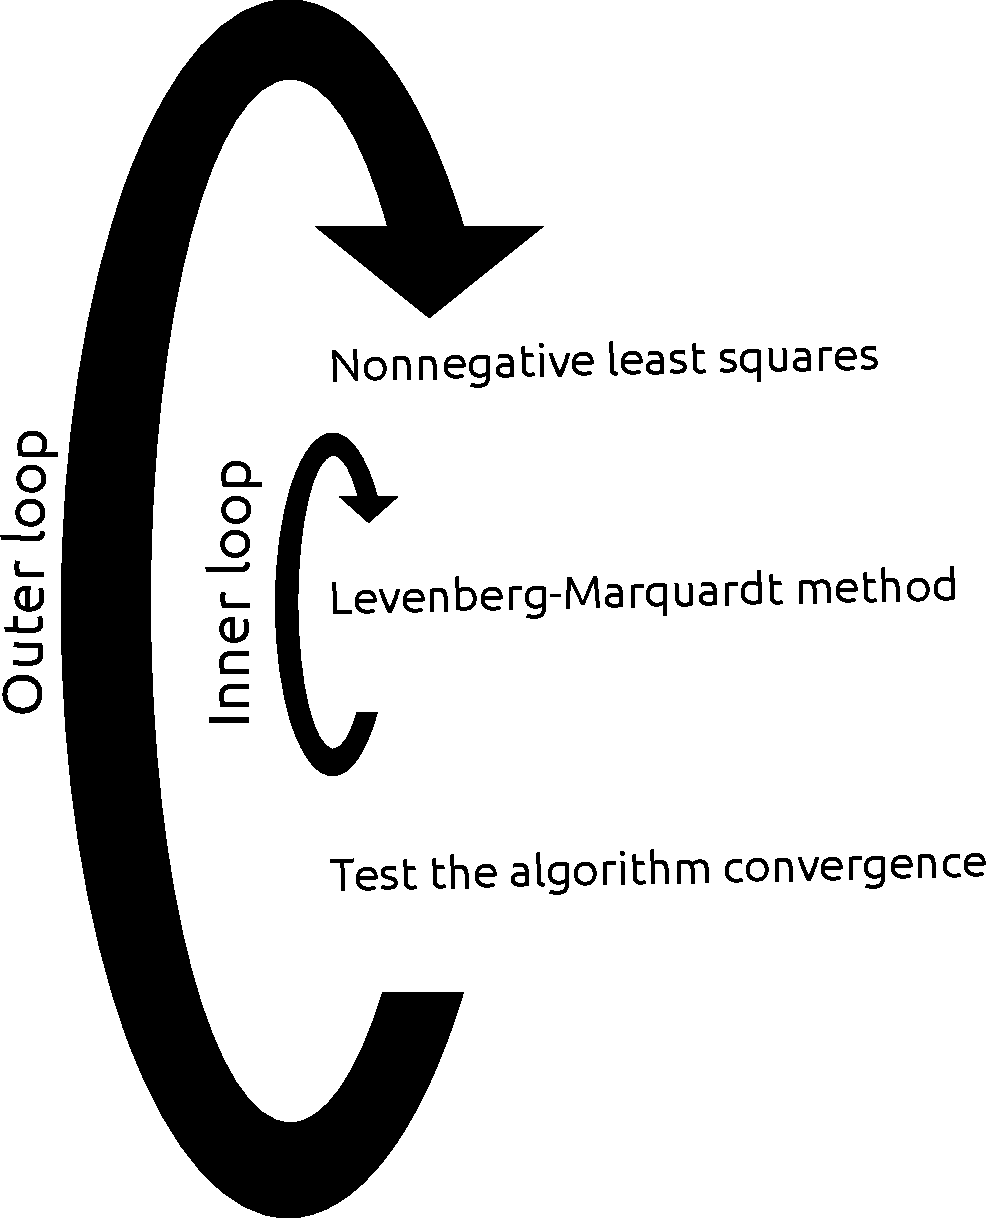
\includegraphics[width=0.6\textwidth]{Fig/algorithm_LM_NNLS.pdf}
	\caption{Iterative scheme overview for NNLS and Levenberg-Marquardt method for estimating magnetization direction. The outer loop is the nonnegative solution for magnetic-moment distribution and the inner loop calculates the magnetization direction correction using Levenberg-Marquardt method.}
	\label{fig:scheme_LM_NNLS}
\end{figure}

%% Figures synthetic tests

\begin{figure}
	\centering
	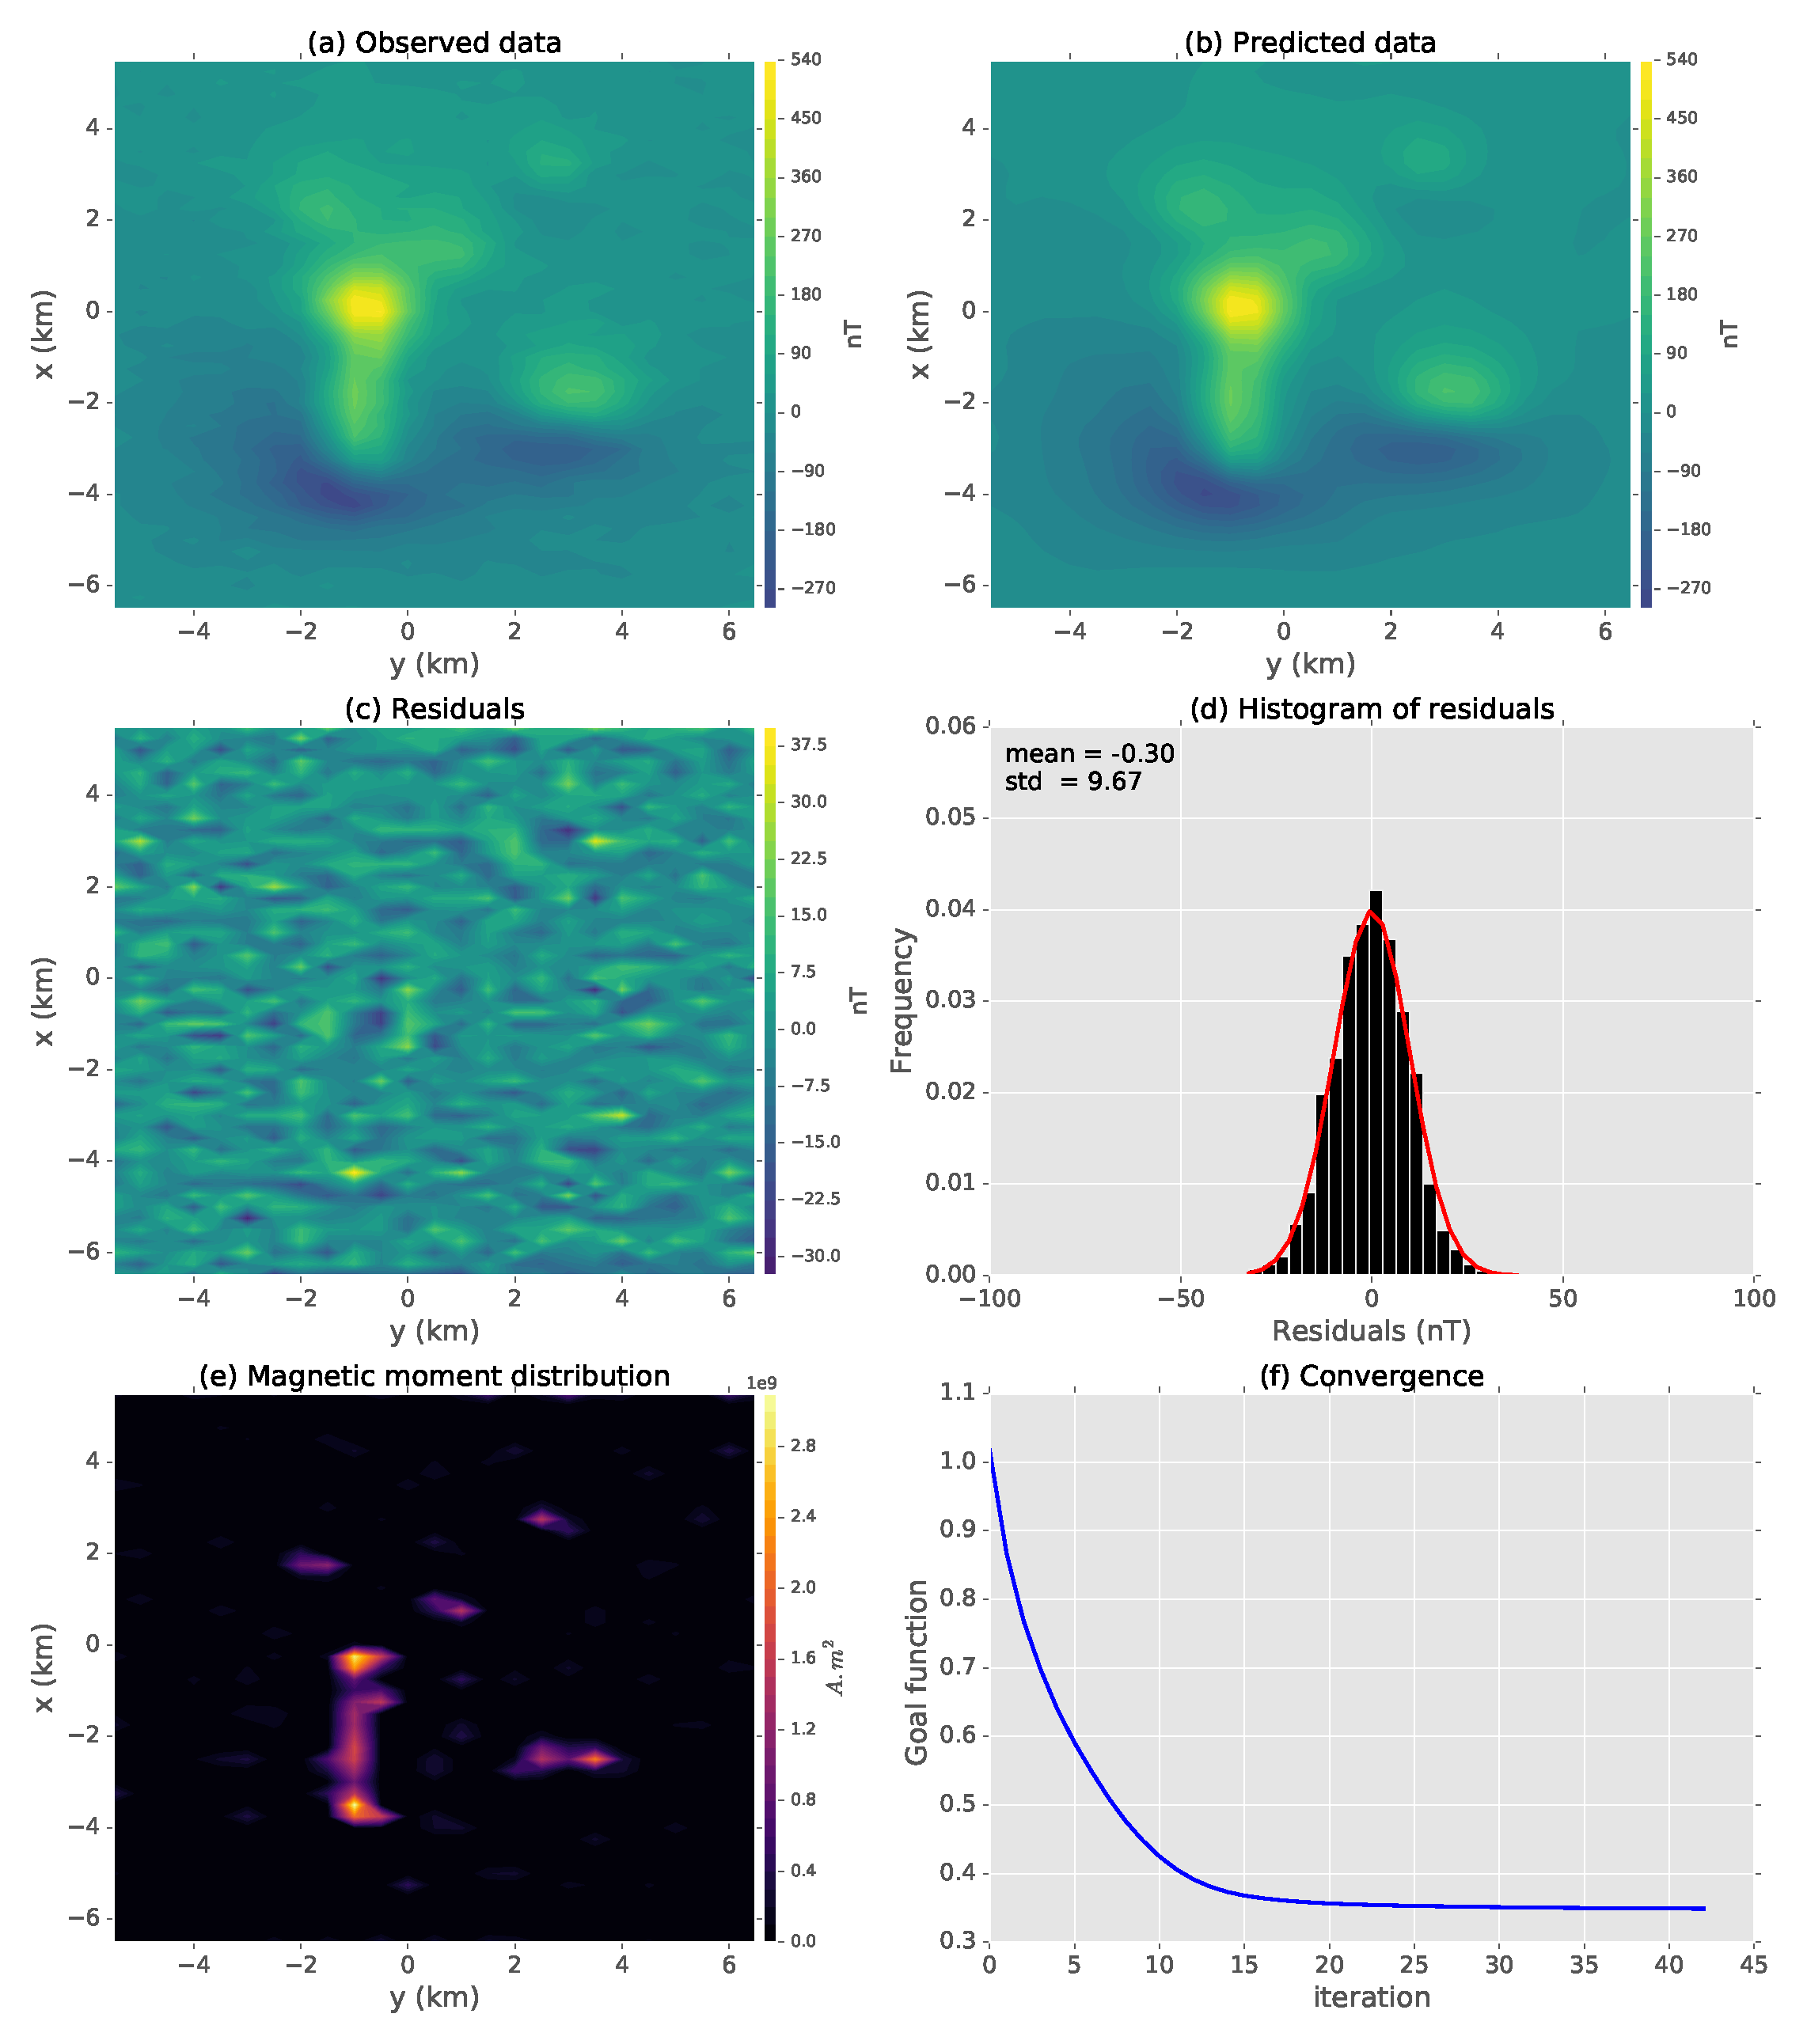
\includegraphics[width=0.85\textwidth]{Fig/unidir_test/results_compiled_LM_NNLS_magRM.eps}
	\caption{Application to synthetic data for unidirectional model. (a) Noise-corrupted data. (b) Predicted data produced by equivalent layer. (c) Difference between the data shown in panels (a) and (b). (d) Histogram of residuals. (e) All-positive magnetic moment distribution. (f) Goal function value (equation \ref{eq:positivity_goal_function}a) per iteration showing the convergence.}
	\label{fig:unidir_test}
\end{figure}

\begin{figure}
	\centering
	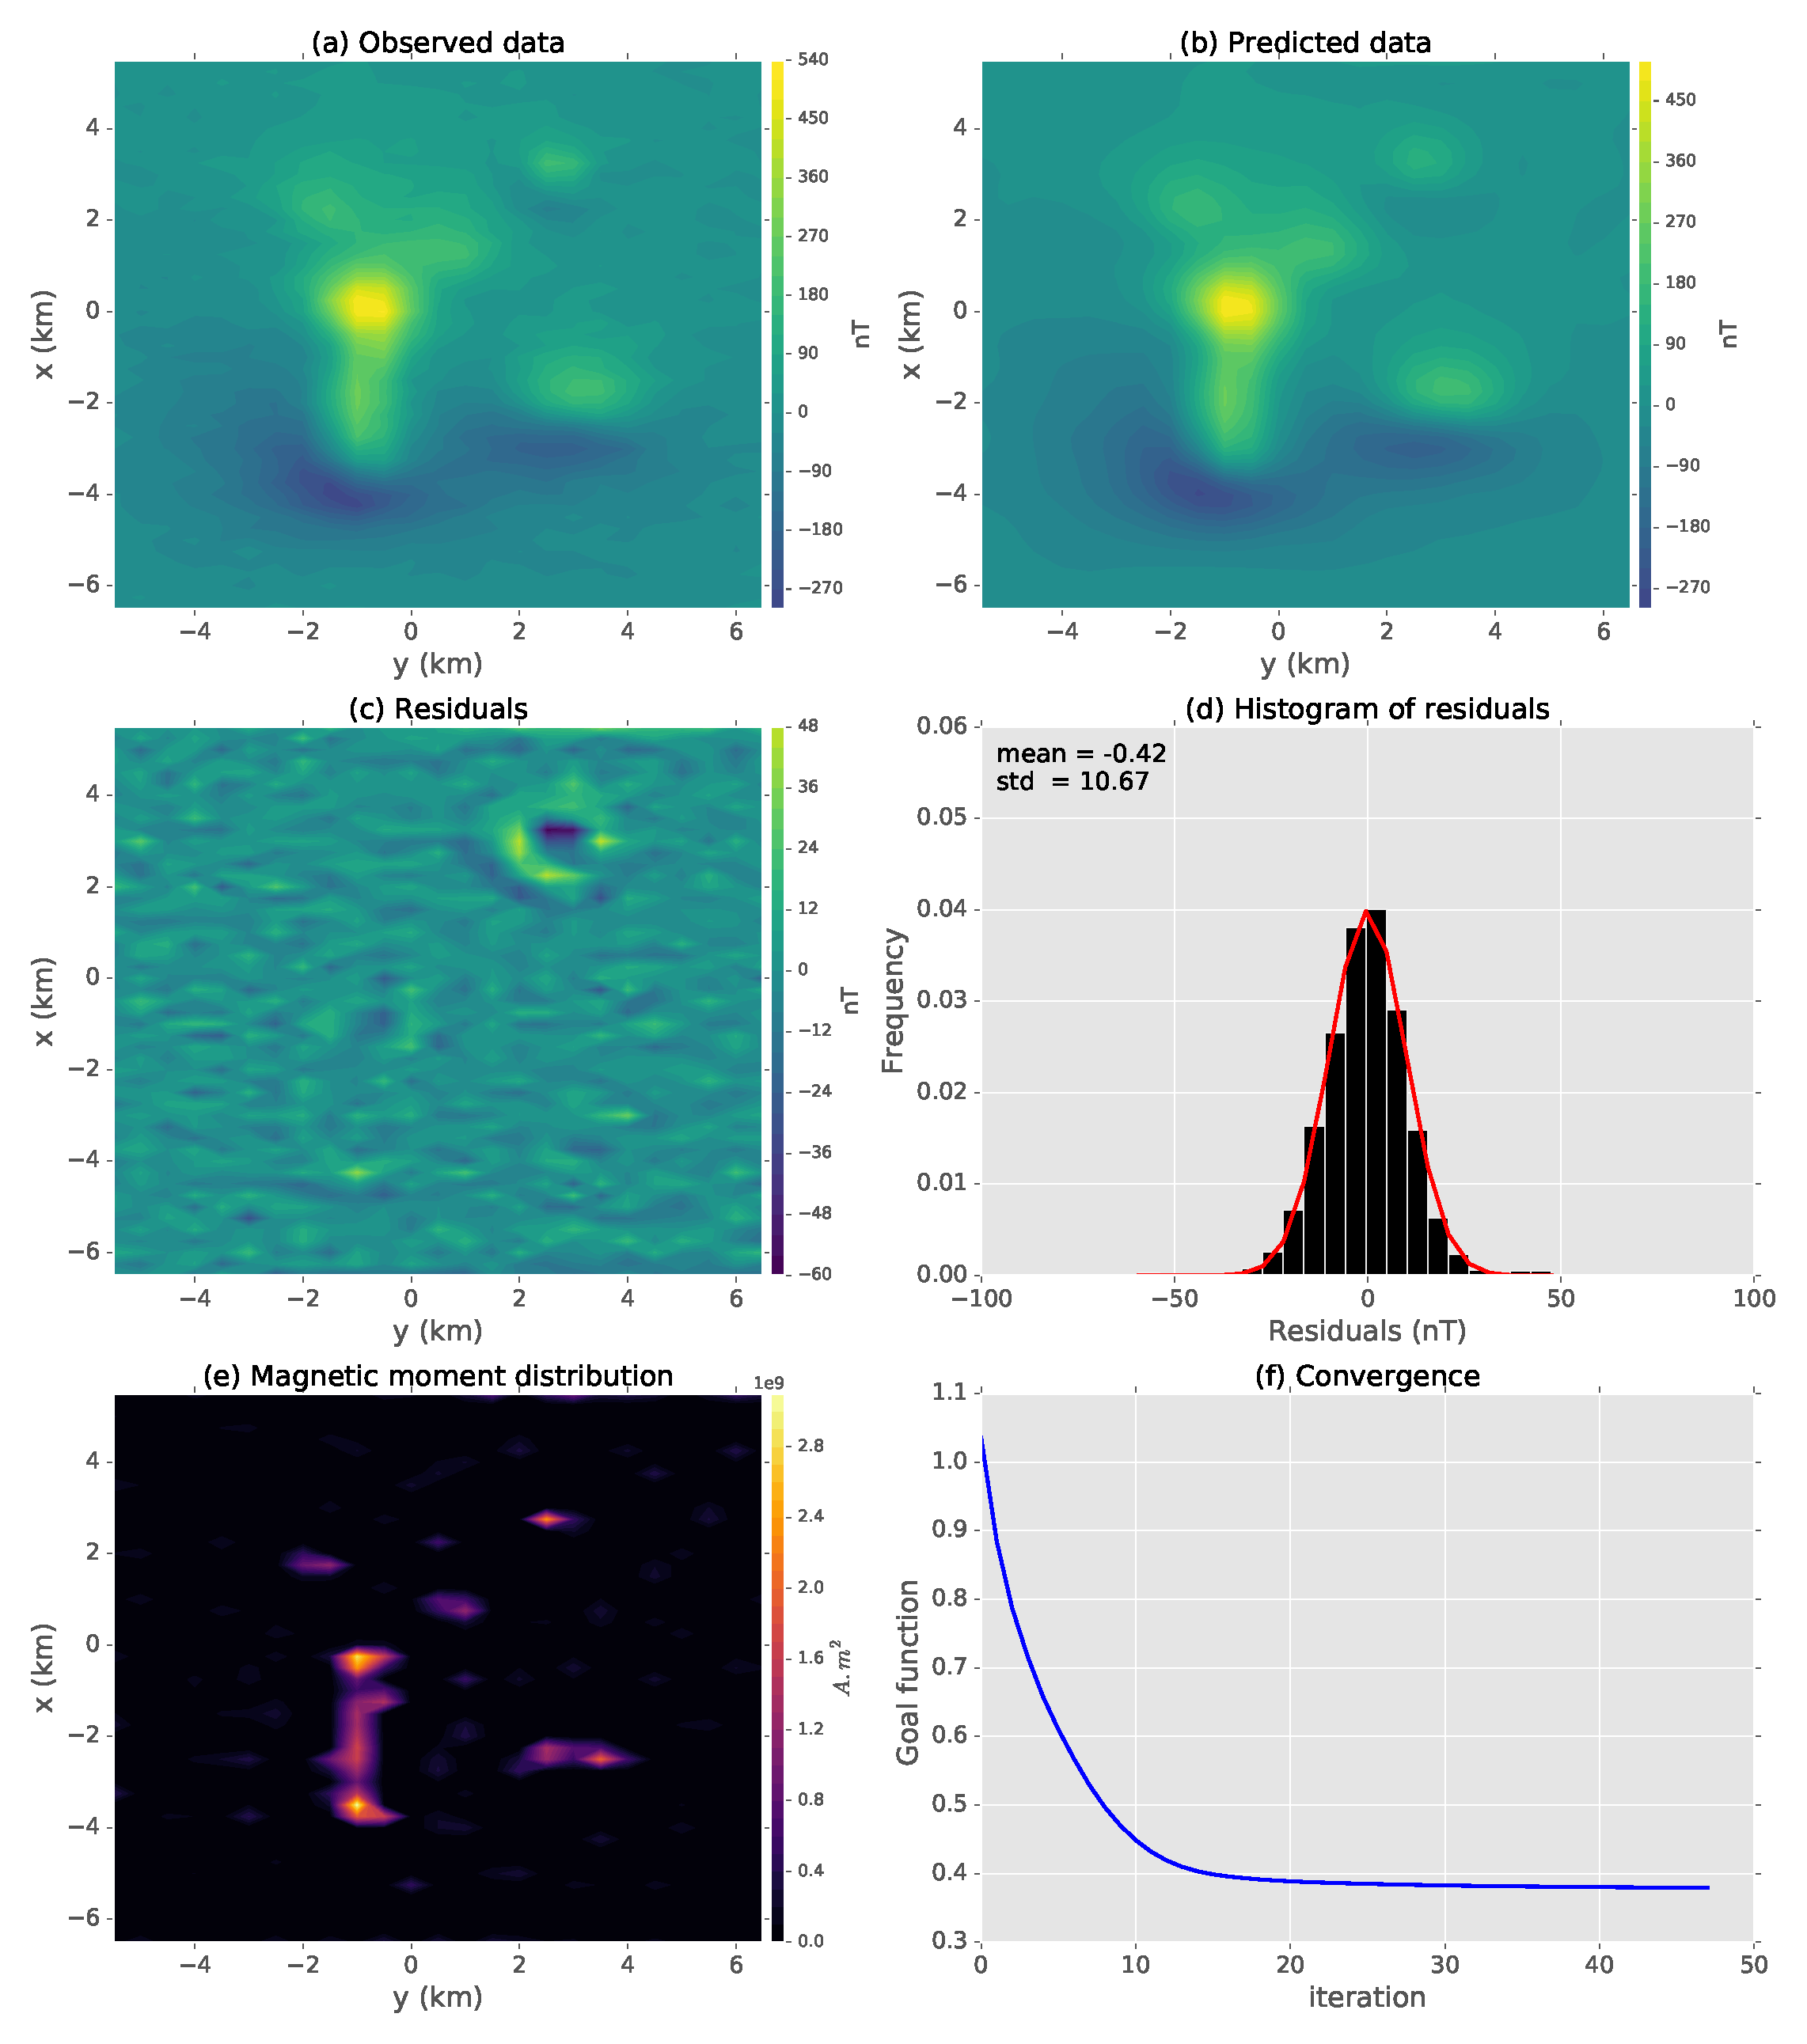
\includegraphics[width=0.85\textwidth]{Fig/unidir_shallow_test/results_compiled_LM_NNLS_magRM.eps}
	\caption{Application to synthetic data with a shallow interfering source. (a) Noise-corrupted data. (b) Predicted data produced by equivalent layer. (c) Difference between the data shown in panels (a) and (b). (d) Histogram of residuals. (e) All-positive magnetic moment distribution. (f) Goal function value (equation \ref{eq:positivity_goal_function}a) per iteration showing the convergence.}
	\label{fig:unidir_shallow_test}
\end{figure}

\begin{figure}
	\centering
	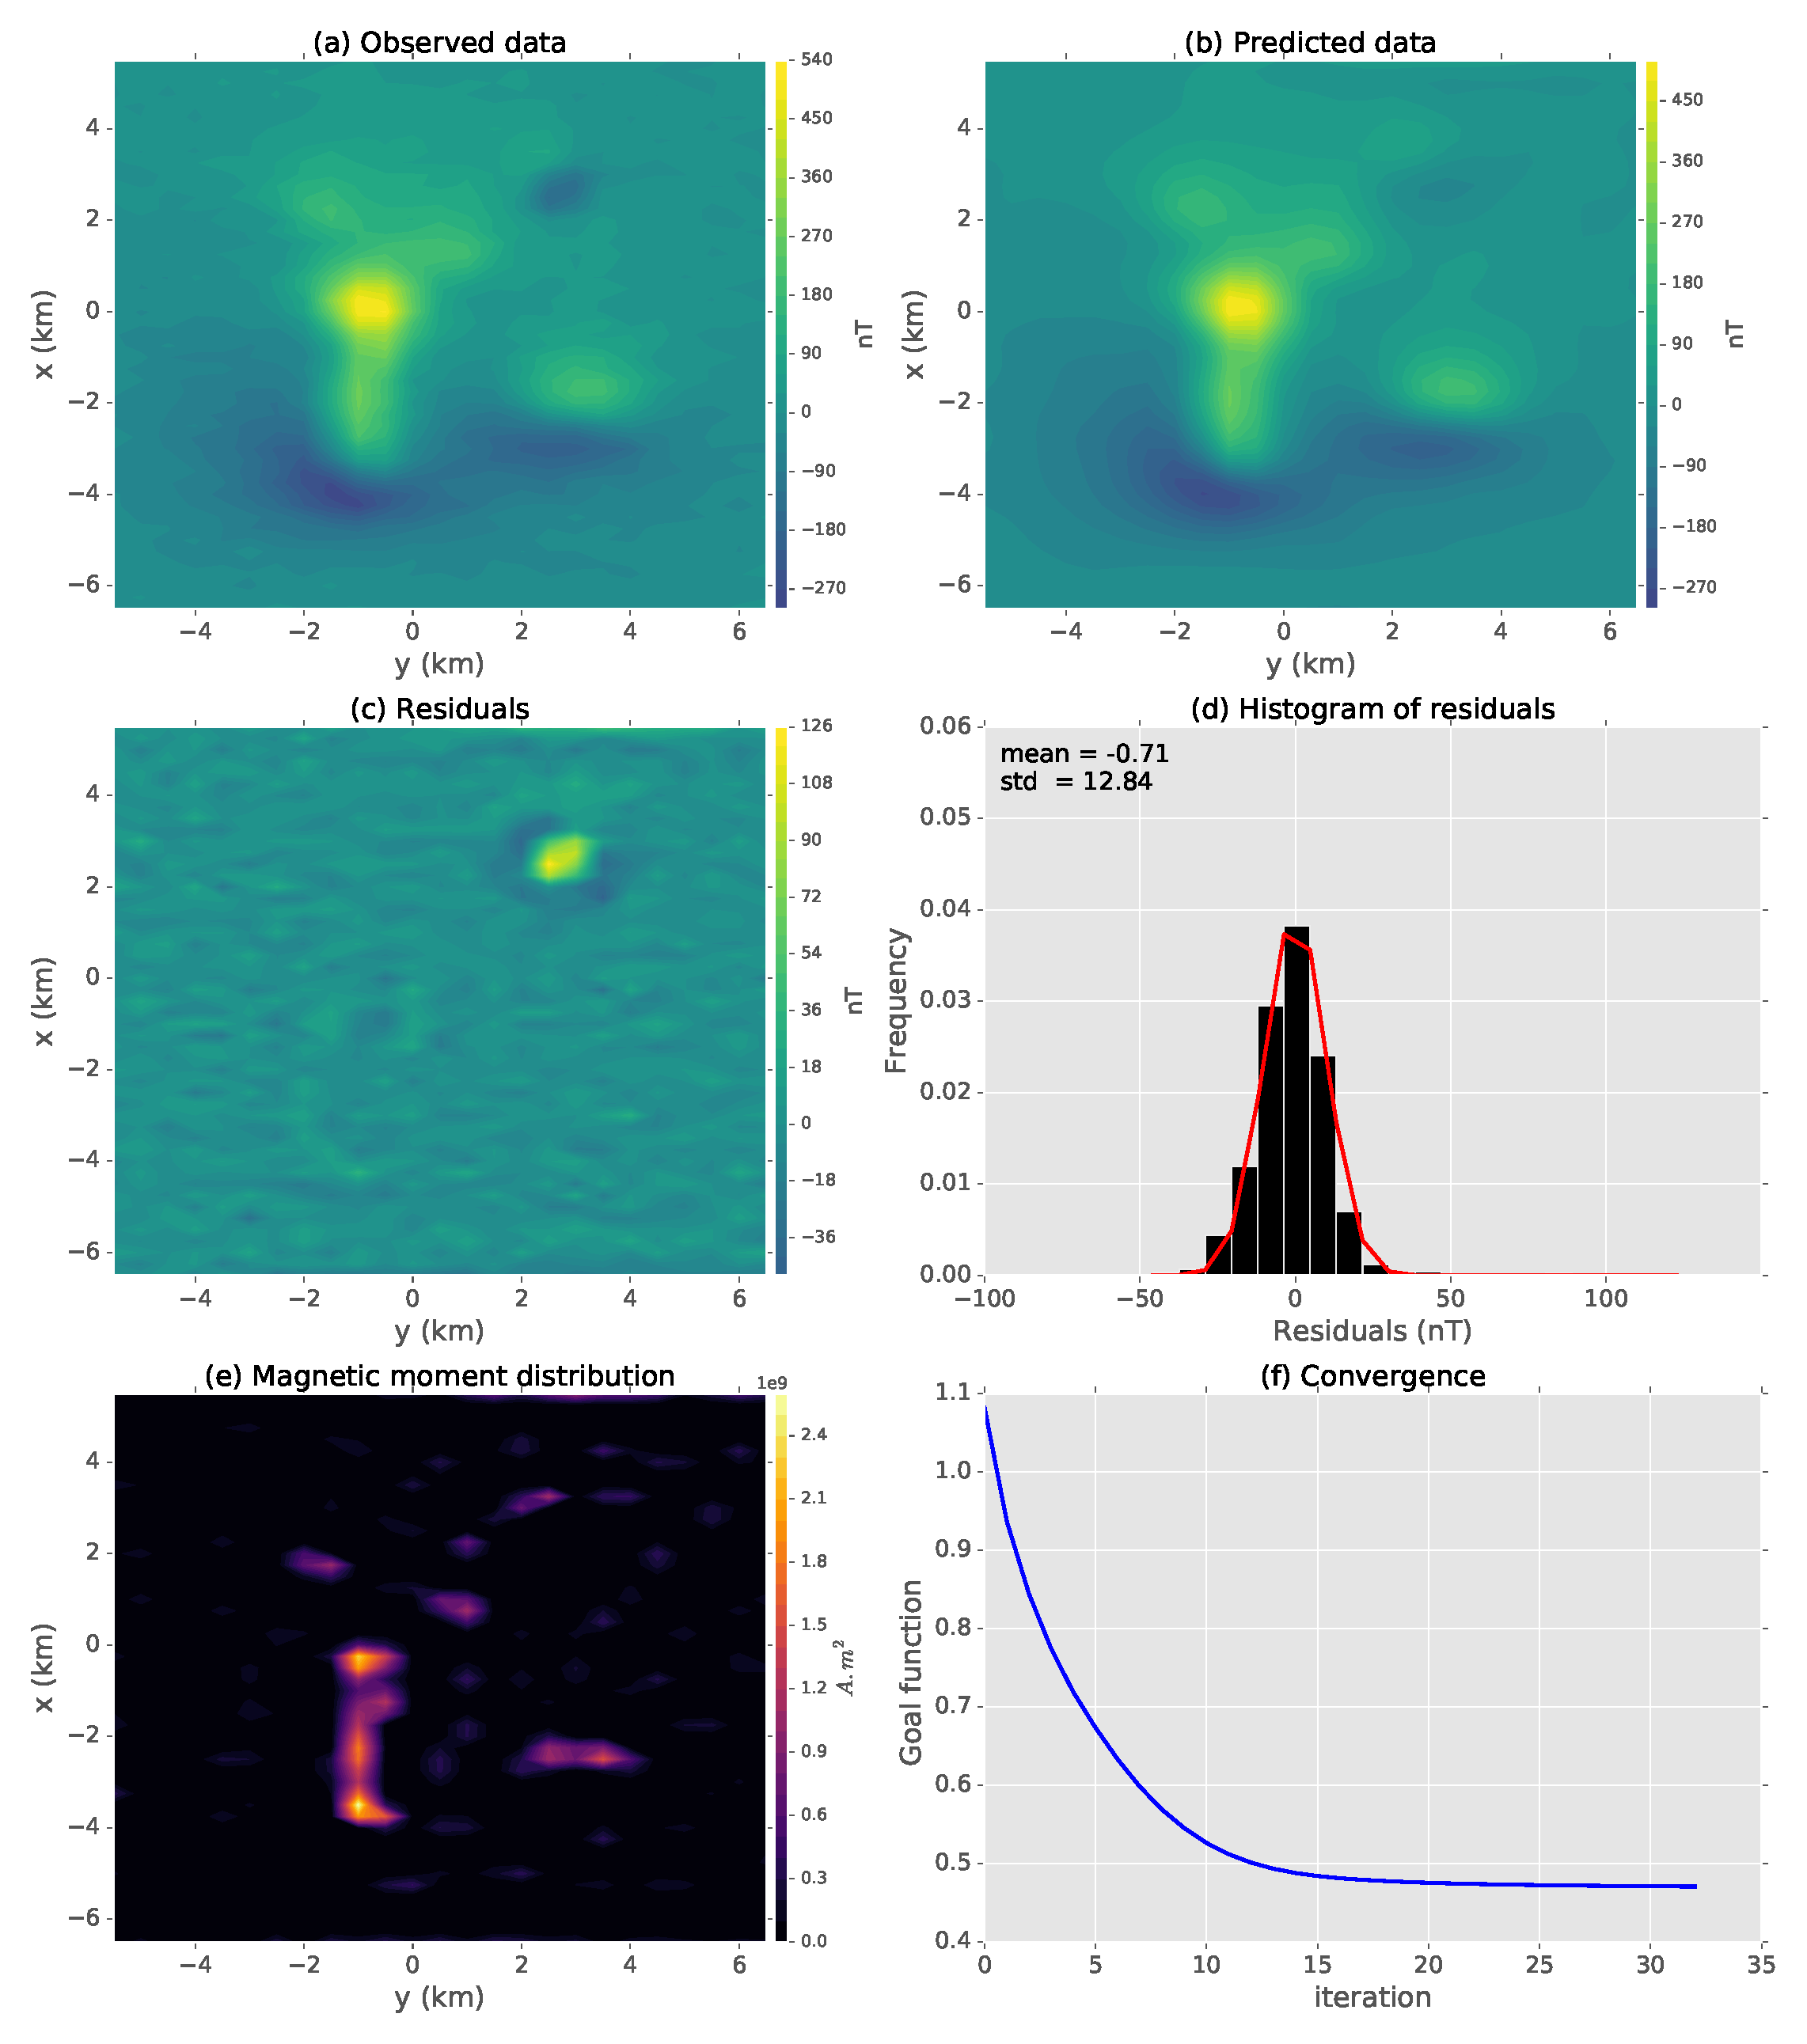
\includegraphics[width=0.85\textwidth]{Fig/unidir_shallow_diff_test/results_compiled_LM_NNLS_magRM.eps}
	\caption{Application to synthetic data with a shallow interfering source with different magnetization direction. (a) Noise-corrupted data. (b) Predicted data produced by equivalent layer. (c) Difference between the data shown in panels (a) and (b). (d) Histogram of residuals. (e) All-positive magnetic moment distribution. (f) Goal function value (equation \ref{eq:positivity_goal_function}a) per iteration showing the convergence.}
	\label{fig:unidir_shallow_diff_test}
\end{figure}

%% Real data application 
\begin{figure}
	\centering
	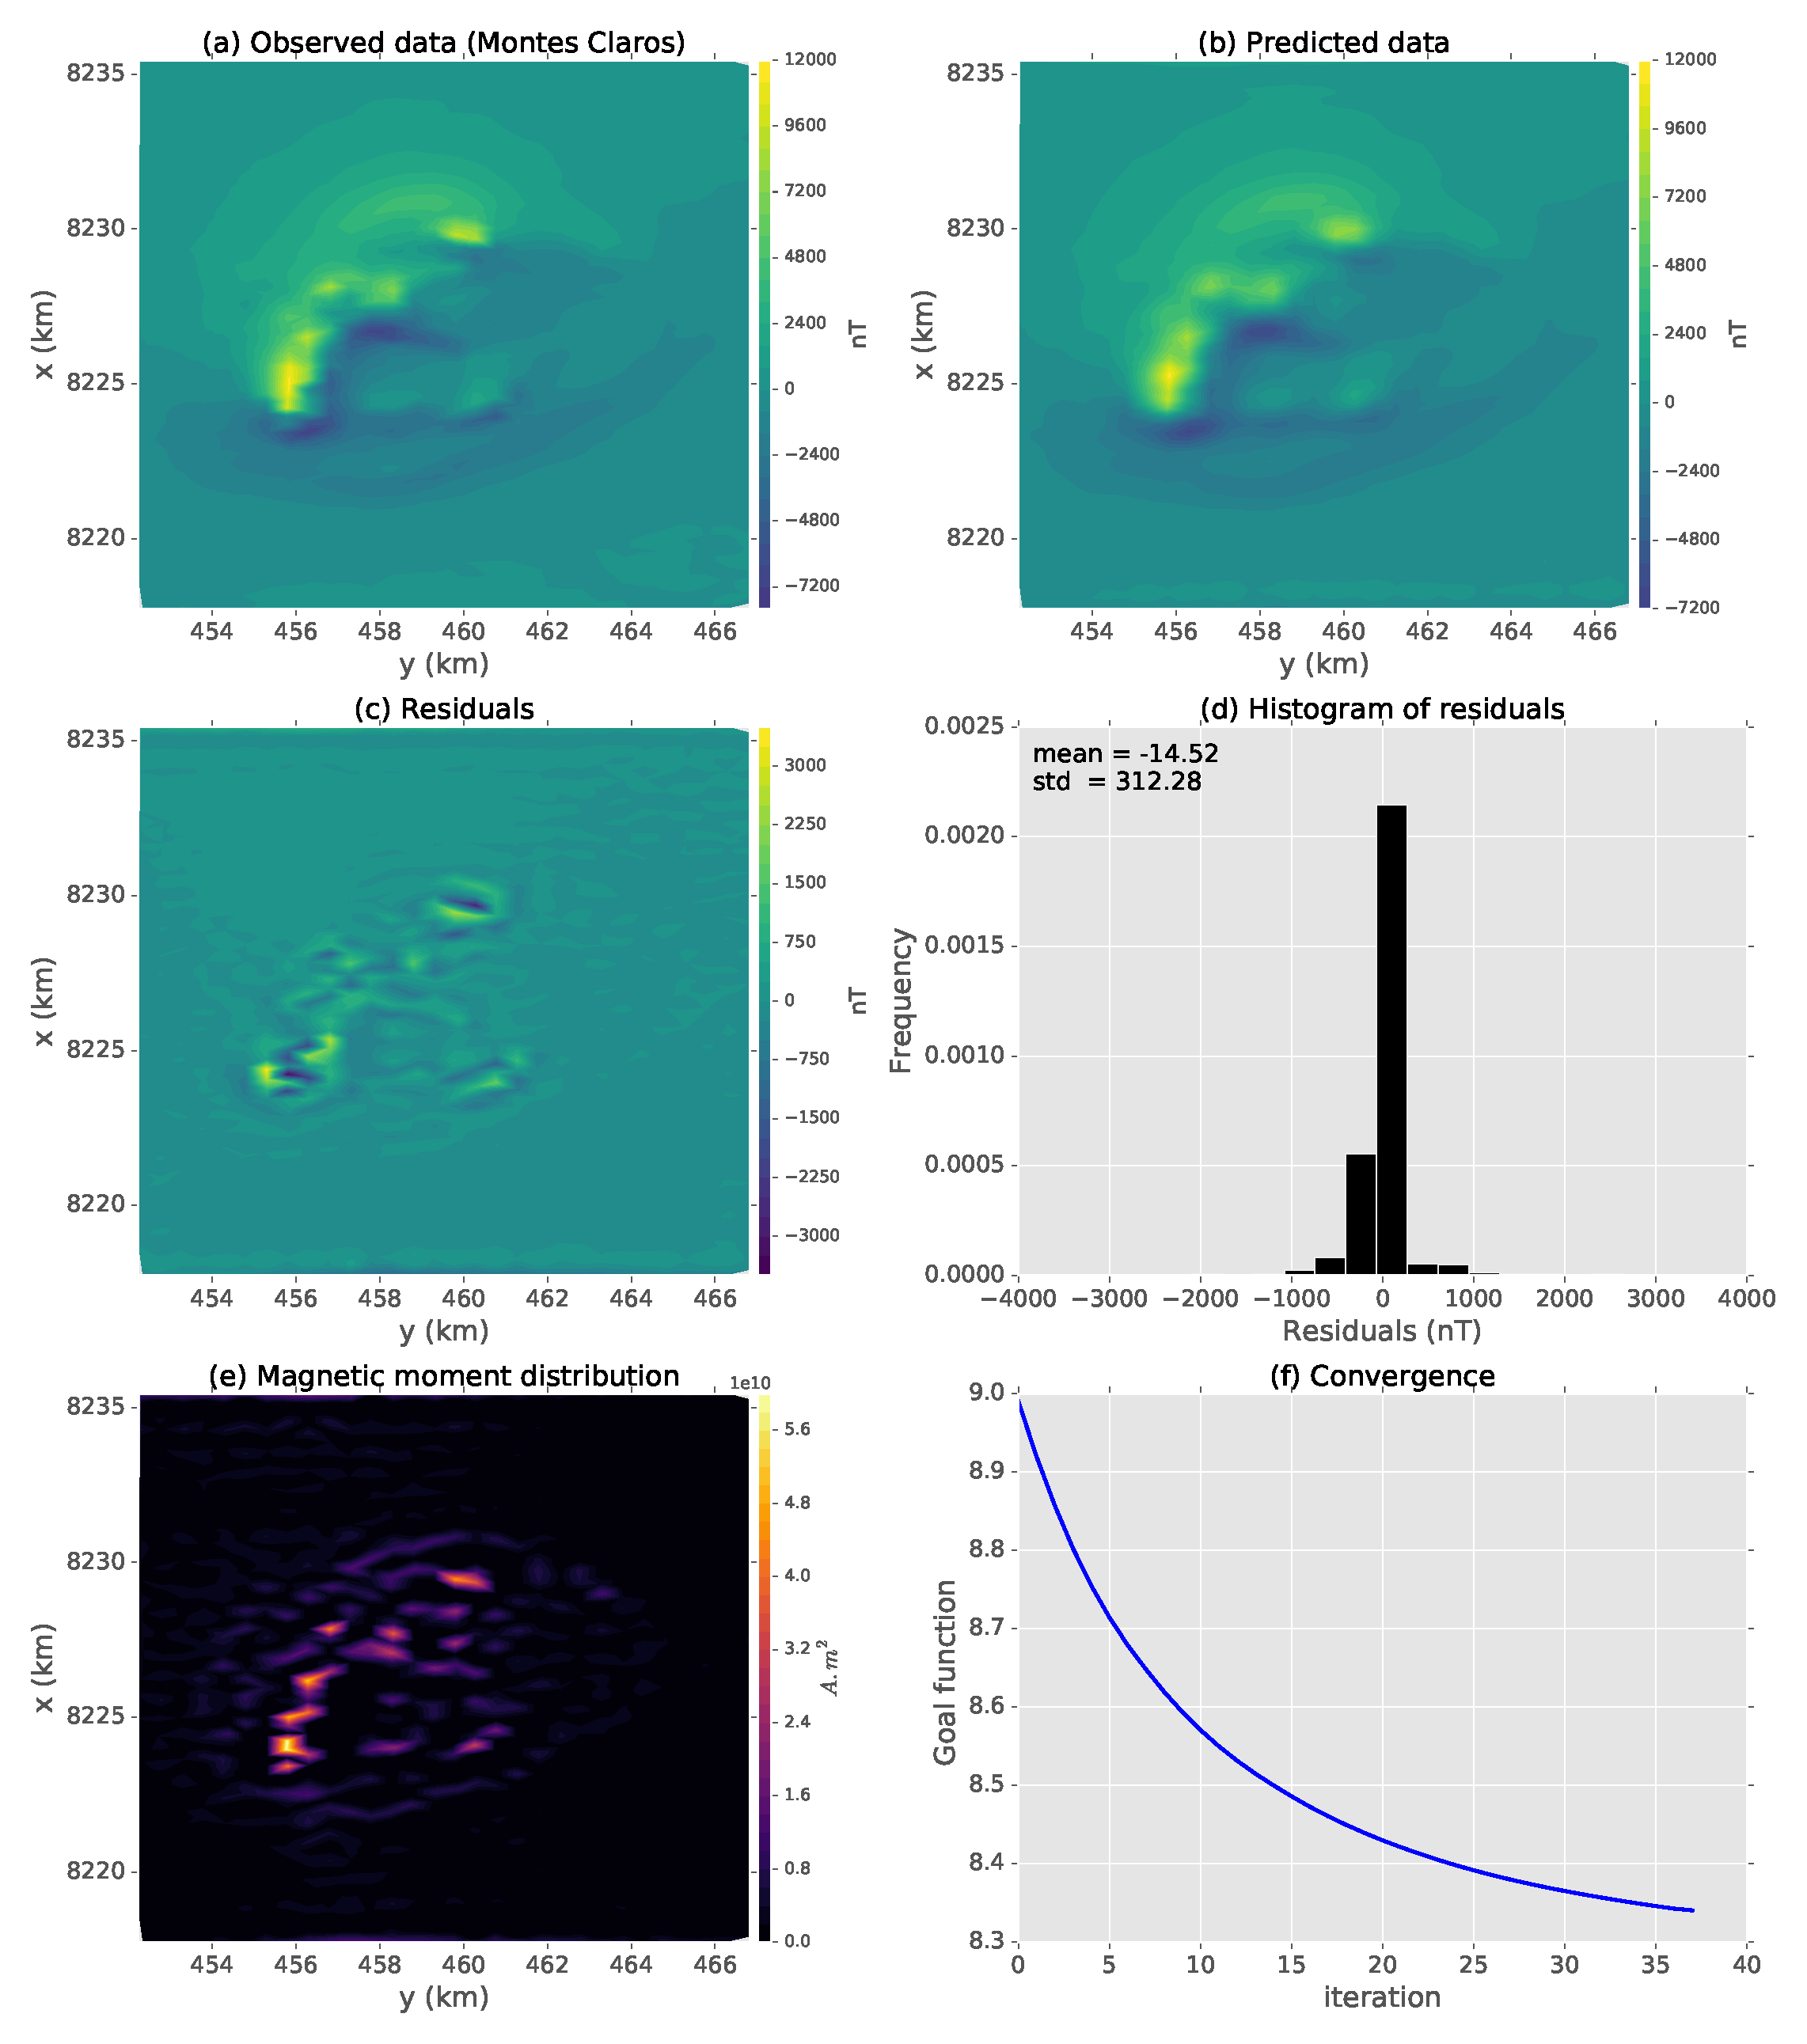
\includegraphics[width=0.85\textwidth]{Fig/field_data_montes_claros/montes_claros_compiled_LM_NNLS_magRM.eps}
	\caption{Application to field data located in complex of Montes Claros. (a) Observation data. (b) Predicted data produced by equivalent layer. (c) Difference between the data shown in panels (a) and (b). (d) Histogram of residuals. (e) All-positive magnetic moment distribution. (f) Goal function value (equation \ref{eq:positivity_goal_function}a) per iteration showing the convergence.}
	\label{fig:mc_data_application}
\end{figure}

\begin{figure}
	\centering
	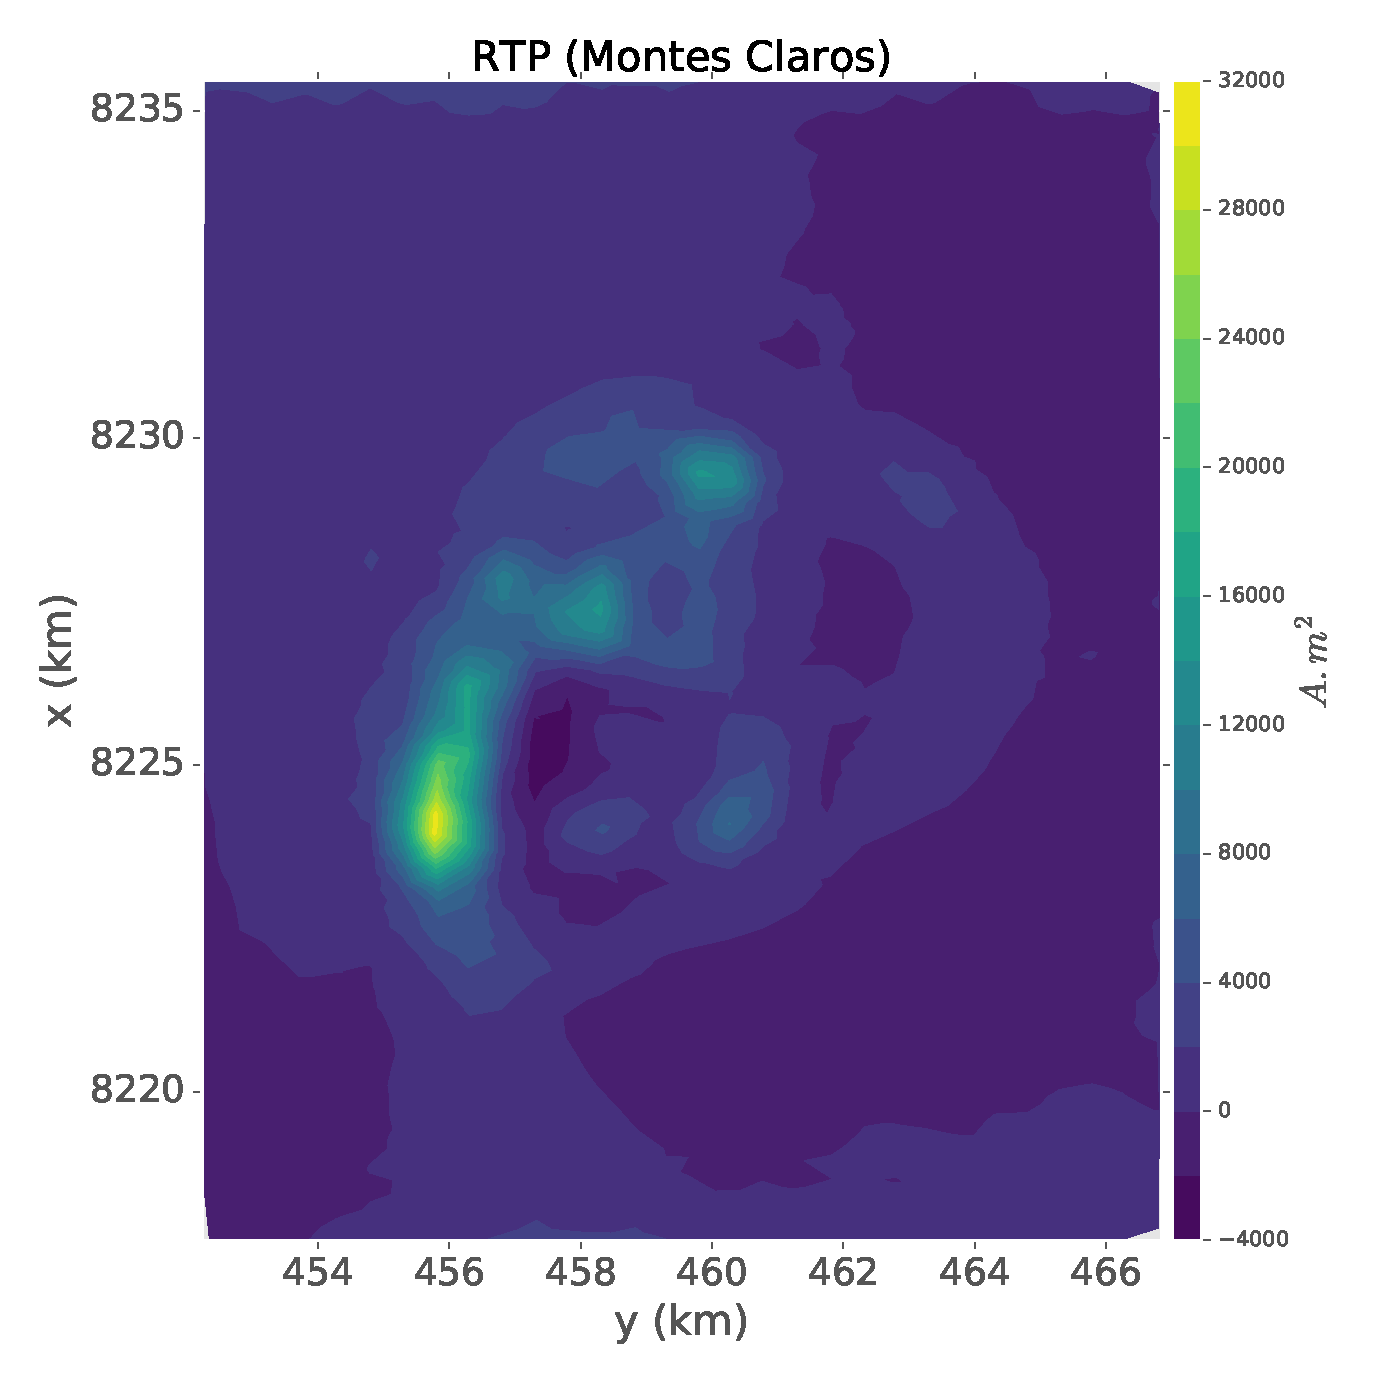
\includegraphics[width=0.75\textwidth]{Fig/field_data_montes_claros/RTP_data_montes_claros.eps}
	\caption{Application to field data located in complex of Montes Claros. RTP anomaly computed by using the estimated magnetization distribution shown in figure \ref{fig:mc_data_application}e.}
	\label{fig:rtp_mc_data}
\end{figure}
